\documentclass[10pt]{article}
% \usepackage[letterpaper]{geometry}
\usepackage[utf8]{inputenc}

\usepackage[margin = 0.5in]{geometry}
\usepackage{graphicx}
% \usepackage{amsmath}
\usepackage{amssymb}
\usepackage{float}
% \usepackage{hyperref}
\usepackage{multicol}
\usepackage{listings}
% \usepackage{minted}
% \usemintedstyle{emacs}

% \usepackage[linesnumbered,ruled,vlined]{algorithm2e}
% Single image

% \begin{figure}[H]
%     \centering
%     \includegraphics[scale = 0.9 ]{ellipse.png}
%     \caption{results/Q1/ellipse.png}
% \end{figure}

% Double images

% \begin{figure}[H]
%     \centering
%     \begin{minipage}{0.49\textwidth}
%     \includegraphics[width =\textwidth]{}
%     \caption{}
%     \end{minipage} \hfill
%     \begin{minipage}{0.49\textwidth}    
%     \includegraphics[width = \textwidth]{}
%     \caption{}
%     \end{minipage}
% \end{figure}
% \usepackage{tikz}
% \usetikzlibrary{automata, positioning, arrows}

% \tikzset{
% ->, 
% >=latex, 
% node distance=3cm, .
% every state/.style={thick, fill=gray!10}, 
% initial text=$ $, 
% }

\newcommand\blfootnote[1]{%
  \begingroup
  \renewcommand\thefootnote{}\footnote{#1}%
  \addtocounter{footnote}{-1}%
  \endgroup
}

\usepackage{xcolor}

\definecolor{backcolour}{rgb}{0.95,0.95,0.92}
\definecolor{codegreen}{rgb}{0,0.6,0}

% Define a custom style
\lstdefinestyle{myStyle}{
    backgroundcolor=\color{backcolour},   
    commentstyle=\color{codegreen},
    basicstyle=\ttfamily\footnotesize,
    breakatwhitespace=false,         
    breaklines=true,                 
    keepspaces=true,                 
    numbers=left,       
    numbersep=5pt,                  
    showspaces=false,                
    showstringspaces=false,
    showtabs=false,                  
    tabsize=2,
}

% Use \lstset to make myStyle the global default
\lstset{style=myStyle}

\definecolor{commentsColor}{rgb}{0.497495, 0.497587, 0.497464}
\definecolor{keywordsColor}{rgb}{0.000000, 0.000000, 0.635294}
\definecolor{stringColor}{rgb}{0.558215, 0.000000, 0.135316}

\title{CS747 Foundation of Learning Agents \\ Assignment 2}
\author{Sanchit Jindal \quad 200020120}
\date{}

\begin{document}
\maketitle

\section{MDP Planning}

To Run:
\begin{verbatim}
    python planner.py --mdp MDPFILE [--algorithm vi/hpi/lp ]/[ --policy POLICYFILE]
\end{verbatim}

\noindent
The Code is available in the file \textbf{planner.py} and I have chosen the Value Iteration algorithm to be the default algorithm \\
I have tried to vectorize the code wherever possible to reduce the time required to run the scripts

\subsection{Value Iteration}
This Algorithm is 
\begin{lstlisting}[escapeinside={|*}{*|}]
    Initialize Value Vector |*$V \in \mathbb{R}^n $*|
    do
        |*$V_{new} \leftarrow \max_{action} \;\sum_{state}\; T\{R + \gamma V\}$*|
        |*$error \leftarrow ||V - V_{new}||$*|
        |*$V \leftarrow V_{new}$*|
    while (error|*$\le \Delta$*|) # A limit parameter
    |*$ \pi \leftarrow arg\,max_{action} \;\sum_{state}\; T\{R + \gamma V\}$*|
    return |*$ V, \pi$*| 
\end{lstlisting}

That is we keep iterating the over the Value function by using the Bellman Optimality Operator till the values converge

\subsection{Howards Policy Improvements}
The Algorithm is 
\begin{lstlisting}[escapeinside={|*}{*|}]
    Initialize policy |*$\pi \in A^n \;\;(A$*| is the set of actions)
    do 
        Initialize Value Vector |*$V \in \mathbb{R}^n $*|
        do
            # Choosing the Values Corresponding to the policies
            |*$V_{new} \leftarrow \sum_{state}\; T\{R + \gamma V\} [\pi]$*|
            |*$error \leftarrow ||V - V_{new}||$*|
            |*$V \leftarrow V_{new}$*|
        while (error|*$\le \Delta$*|) # A limit parameter
    
        |*$ \pi \leftarrow arg\,max_{action} \;\sum_{state}\; T\{R + \gamma V\}$*|
    while (policy Changed)
    return |*$ V, \pi$*| 
\end{lstlisting}
That is we choose a arbitary policy and calculate the Value Function for each state.
Then We check if there exists a policy that can give a better value function by applying the Bellman Operator.
If True then we repeat with the new better policy till there is no change. 
As we are choosing argmax over all the actions if a state is improvable it is being improved.

\subsection{Linear Program}
We are solving the Problem
\begin{lstlisting}[escapeinside = {!}{!}]
    !$MAX_{V} \quad \sum V$ !
    s.t     
        !$ V(s) \ge \sum T\{R + \gamma V\} \quad \forall s, \forall a $! 
\end{lstlisting}

The Problem is solved using the \verb|PulP| library of python 
As we need to create a PulP Equation The Code could not be vectorized 

\subsection{Policy Evaluation}
The Policy Evaluation is same as the Value Computation code in the Howards Policy Iteration.


\blfootnote{The --policy and --algorithm flags for the planner.py are mutually exclusive, so if policy given algorithm is ignored.}
\begin{lstlisting}[escapeinside={|*}{*|}]
Given policy |*$ \pi $*|
    Initialize Value Vector |*$V \in \mathbb{R}^n $*|
    do
        # Choosing the Values Corresponding to the policies
        |*$V_{new} \leftarrow \sum_{state}\; T\{R + \gamma V\} [\pi]$*|
        |*$error \leftarrow ||V - V_{new}||$*|
        |*$V \leftarrow V_{new}$*|
    while (error|*$\le \Delta$*|) # A limit parameter
    return |*$V$*| 
\end{lstlisting}

\subsection{Utilitities}
To Better Organize the Code:-

\begin{itemize}
    \item I have constructed a MDP class that initializes the Transition and Reward matrix with the given values
    \item Both the Matrix are of dimension equivalent to state $\times$ action $\times$ state
    \item The End States are being stored but they are not required as the transition probability value will be zero for them
    \item Similarly the algorithms are applicable for both Continous and Episodic MDPs and is thus not required 
\end{itemize}

\section{MDP for cricket game}

The Commands to run the code are:-
\begin{verbatim}
    python encoder.py --states STATEFILE --parameter PARAMETERFILE --q NUM > MDPFILE
    python planner.py --mdp MDPFILE > VALUEPOLICYFILE
    python decoder.py --value-policy VALUEPOLICYFILE --states STATEFILE
\end{verbatim}

\subsection{Encoder}
I have used the following encoding to produce an MDP

\begin{itemize}
    \item Using the states file I create 2 sets of states by adding a \textbf{O} or a \textbf{1} to the start of the state to denote the 2 batsman.
    \item There are 2 other Terminal states one corresponding to winning the match and the other corresponding to losing.
    \item I map all the different states to  a number from $0$ to NumStates
    \item I also map the possible actions $0,1,2,4,6$ to the numbers $0,1,2,3,4$ as the Planner expects then to be in this fashion.
    \item I make transitions from each states for all possible actions, reading the parameters for the better batsman and using \textit{q} for the tail ender.
    \item For each state for each action the destination is state with one ball less and runs required decreased by runs scored.
    \item To accomodate the possibility that the player may go from one state to another by two possible paths for eg if 2 runs are required and player tries a 6 then on both 4 and 6 runs he reaches the winning terminal state. I had to change the planner.py file to add the transition probability instead of overwriting them
    \item If runs reach less than or equal to zero then the destination is the winning state and reward is one.
    \item If the balls reach zero before or the player gets out then the final state is the losing Terminal state.
    \item Similarly for the tail ender.
    \item The strike changes when player scores 1 or 3 runs.
    \item The strike also changed when the number of balls go from 7 to 6 or 13 to 12
\end{itemize} 

\subsection{Decoder}
The Decoder Assumes that the first lines of the value-policy file correspond to the states in the given file 
And hence it reverse maps the actions and provide the results in the required format

\subsection{Analysis}

To collect and plot data I have used two python scripts
\begin{itemize}
    \item \textbf{collectData.py} It has different blocks of code that can be uncommented to run the other files and generate the values.
    \item \textbf{plot.py} It is a python script plots the data on the basis of two files 
\end{itemize}

\subsubsection{Value Of q}
\textit{The value of q is ranging from 0 to 1 and there are 100 data points}
\begin{figure}[H]
    \centering
    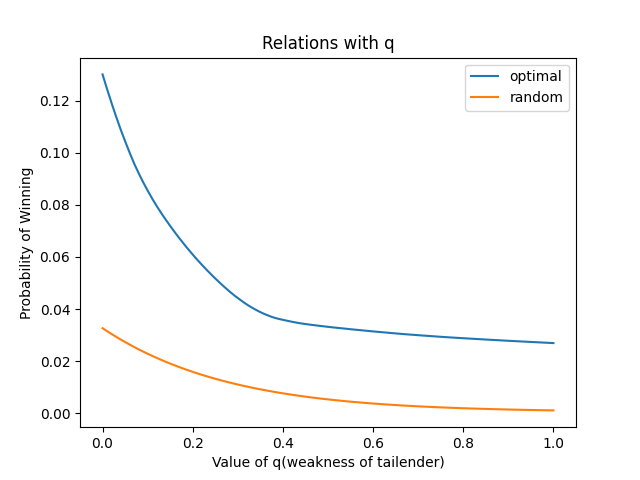
\includegraphics[scale = 0.9 ]{../Figure_1.png}
    \caption{Dependence on q}
\end{figure}


\vspace*{1em}
The Main observations are
\begin{itemize}
    \item The probability of winning the match is always higher if the optimal policy is used, this is to be expected as we optimized the policy to give the most probability.
    \item The Other observations is that the probability reduces as the value of \textbf{q} increases, This is also expected as q is the weakness coffecient and if it is higher than the other player is weaker and hence the probability of winning will be less.
\end{itemize}

\begin{minipage}{0.9\textwidth}
    \subsubsection{Number of Runs Required}
    \textit{There are 10 balls left, q is set to 0.25, and the number of runs required is ranging from 20,19 \dots 1 }
    \begin{figure}[H]
    \centering
    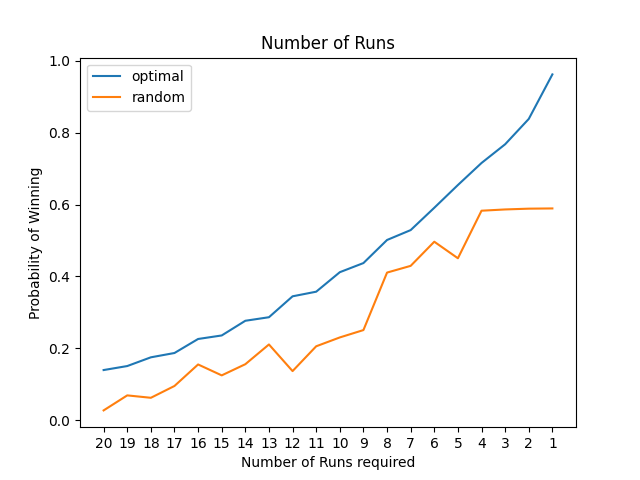
\includegraphics[scale = 0.9 ]{../Figure_2.png}
    \caption{Target to Achive}
\end{figure}
\end{minipage}

The observations from the graph are:
\begin{itemize}
    \item Again the probability of winning is higher if the player followes the optimal policies.
    \item The Probability of winning increases if the number of runs required Decreases, This is expected it will become easier to win if the number of runs required is less.
    \item We can see that the probabililty of winning with the random policy fluctuates much more than the optimal as the random policy though benefitting from the less number of runs required is not able to fully utilize that.
\end{itemize}

\begin{minipage}{0.9\textwidth}
    \subsubsection{Number of Balls Left}
    \textit{10 runs are required, the value of q is again 0.25 and the number of balls left is changed from 15,14 \dots 1}
    \begin{figure}[H]
    \centering
    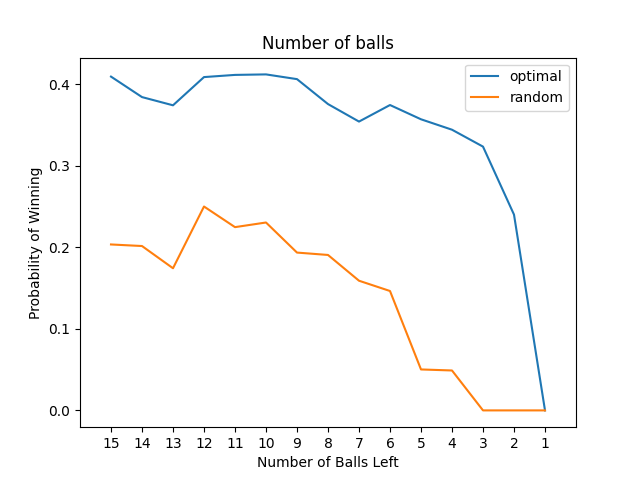
\includegraphics[scale = 0.9]{../Figure_3.png}
    \caption{Balls Left}
\end{figure}
\end{minipage}

The observations are:-
\begin{itemize}
    \item Again the Probability of winning is more for the optimal policy, than the random policy,
    \item The probability decreases as the number of balls left decreases, this is again expected as if there are less number of balls then it is more difficult to win
    \item We can see that the probability of winning is zero if only one ball is left as it is impossible to make 10 runs in one ball.
    \item There probabililty increases a little when the balls left are 12 and 6 as the chance of the strike going to the weaker player is reduced.
\end{itemize}

\section{Submitted files}
The Folder Structure is:-
\begin{verbatim}
submission/
    |-- collectData.py
    |-- decoder.py
    |-- encoder.py
    |-- planner.py
    |-- plot.py
    |-- references.txt
    |-- report.pdf
\end{verbatim}




\end{document}